\citet{Ref64} first suggested that strong lens time delays could be
used to measure absolute distances out to cosmological distances, and
therefore the Hubble Constant to leading order. Unfortunately, no
strong lensing systems were known at that time, and therefore his
intuition remained purely theoretical for over a decade.

The prospects of using time delays for cosmography suddenly brightened
in the late seventies, with the discovery of the first strongly lensed
quasars \citep{WCW79}. Even though they were not the strongly lensed
supernovae that Refsdal had in mind, quasars fluxes are sufficiently
variable \citep{Van82} that people were able to start to put Refsdal's
idea in practice \citep{Van89}. For completeness, we should mention
that the first multiply imaged supernova has been discovered in 2014,
fifty years afer Refsdal's initial suggestion \citep{Kel++15}, lensed
by a foreground cluster of galaxies. The time delays are being
measured at the time of writing
\citep{Rod++16,Kel++16}. However, it is unclear at the moment whether the
cluster potential can be constrained with sufficient precision to
yield interesting cosmological information \citep{Tre++16}. Therefore,
in this review, we will restrict our case to the much more common and
better understood case of a variable quasar being lensed by a
foreground elliptical galaxy.

Discovery and monitoring of lensed quasars continued in the eighties and
nineties, powered by heroic efforts. By the end of the millennium the
number of known strongly lensed systems was in double digits
\citep{CSS02}, and the first truly robust time delays were measured
\citep{Kun++97,Sch++97}.

The discovery of multiply imaged quasars finally took off at the
beginning of the current Millennium with the improvement of panoramic
search technology in dedicated or existing surveys
\citep{Bro++03,Oguri:2006p5865,Agn++15}.

The period of time delay cosmography was marred by controversies over
systematic errors.  The measurement of time delays was particularly
controversial during the nineties as the quality of the early data
allowed for multiple values \citep{PRH92}, owing to the combined
effects of gaps in the data, and microlensing noise in the optical
light curves. This problem was definitely solved at the turn of the
millennium, with the beginning of modern monitoring campaigns,
characterized by high cadence, high precision, and long duration, both
at optical and radio wavelengths
\citep{Fas++99,Fas++02,Bur++02,Eig++05}, as illustrated in Figure~\ref{fig:oldvsmoderndt}. We discuss in more detail
modern monitoring campaigns in Section~\ref{ssec:timedelay}.

\begin{figure*}
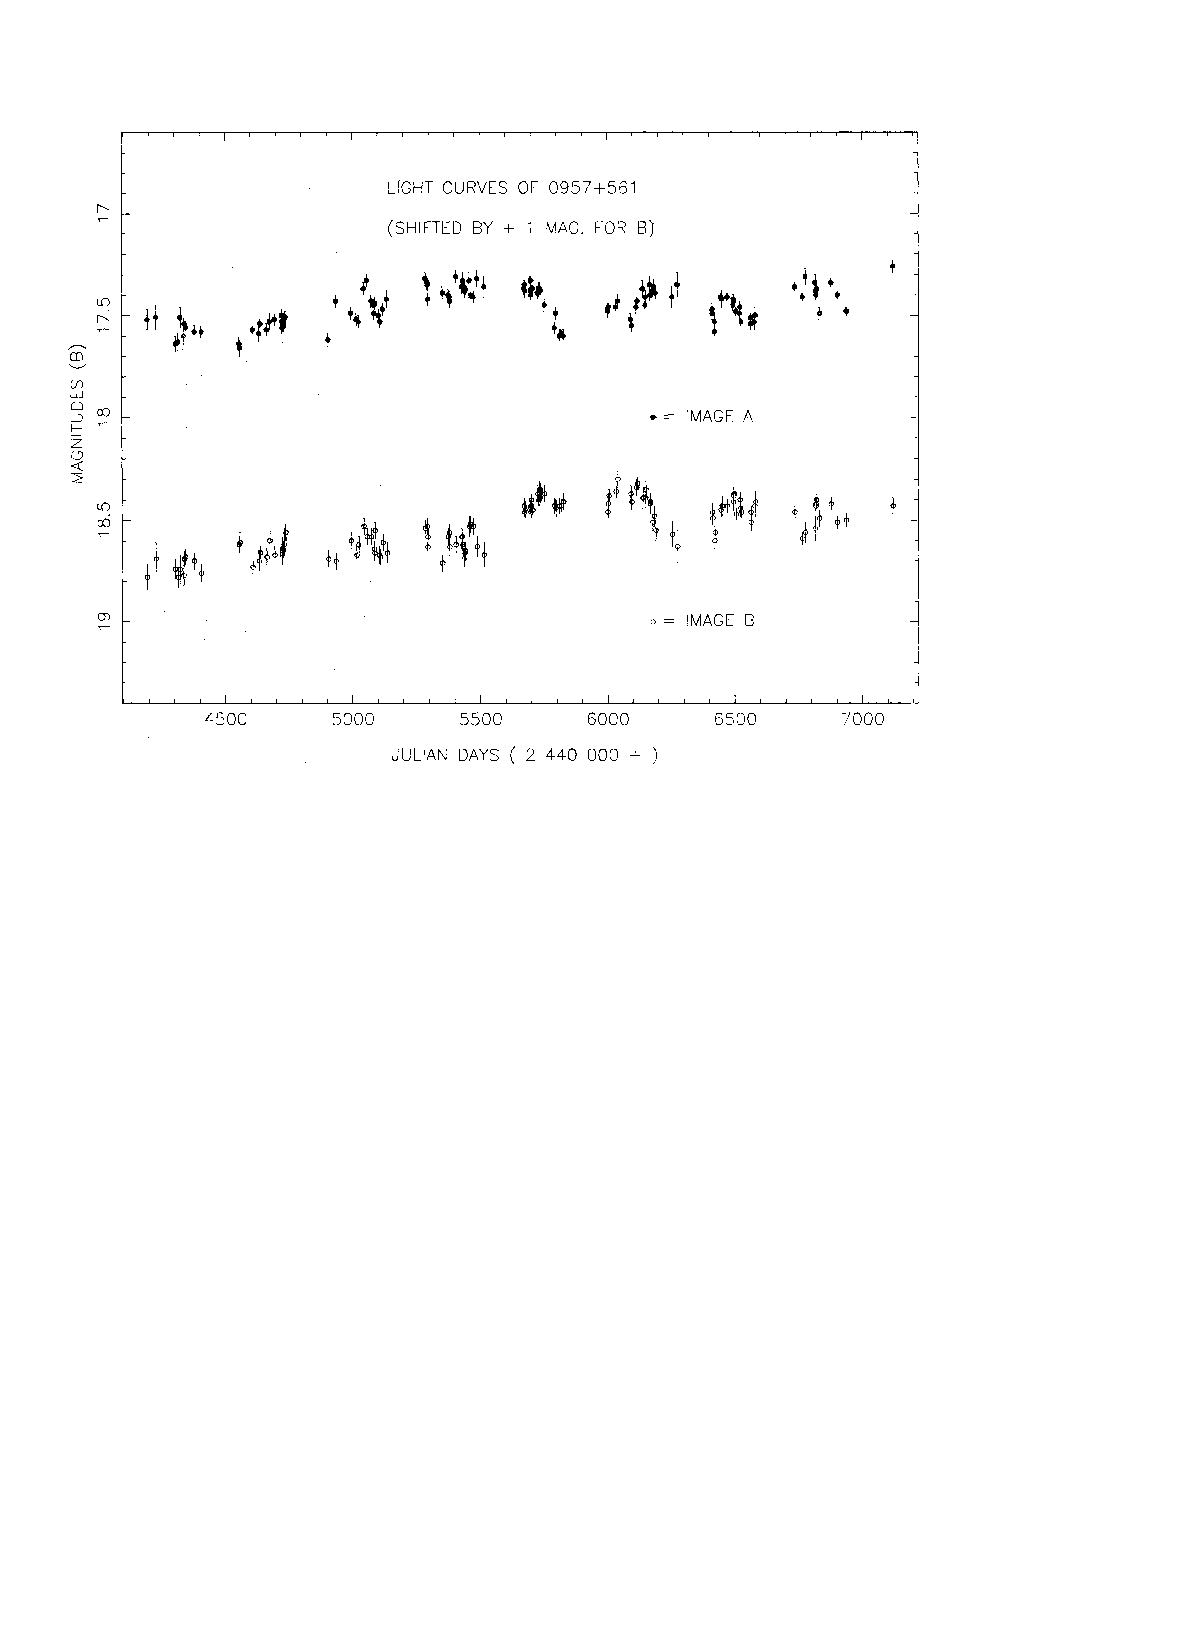
\includegraphics[width=0.48\textwidth]{figures/Vanderriest89_fig5.pdf}
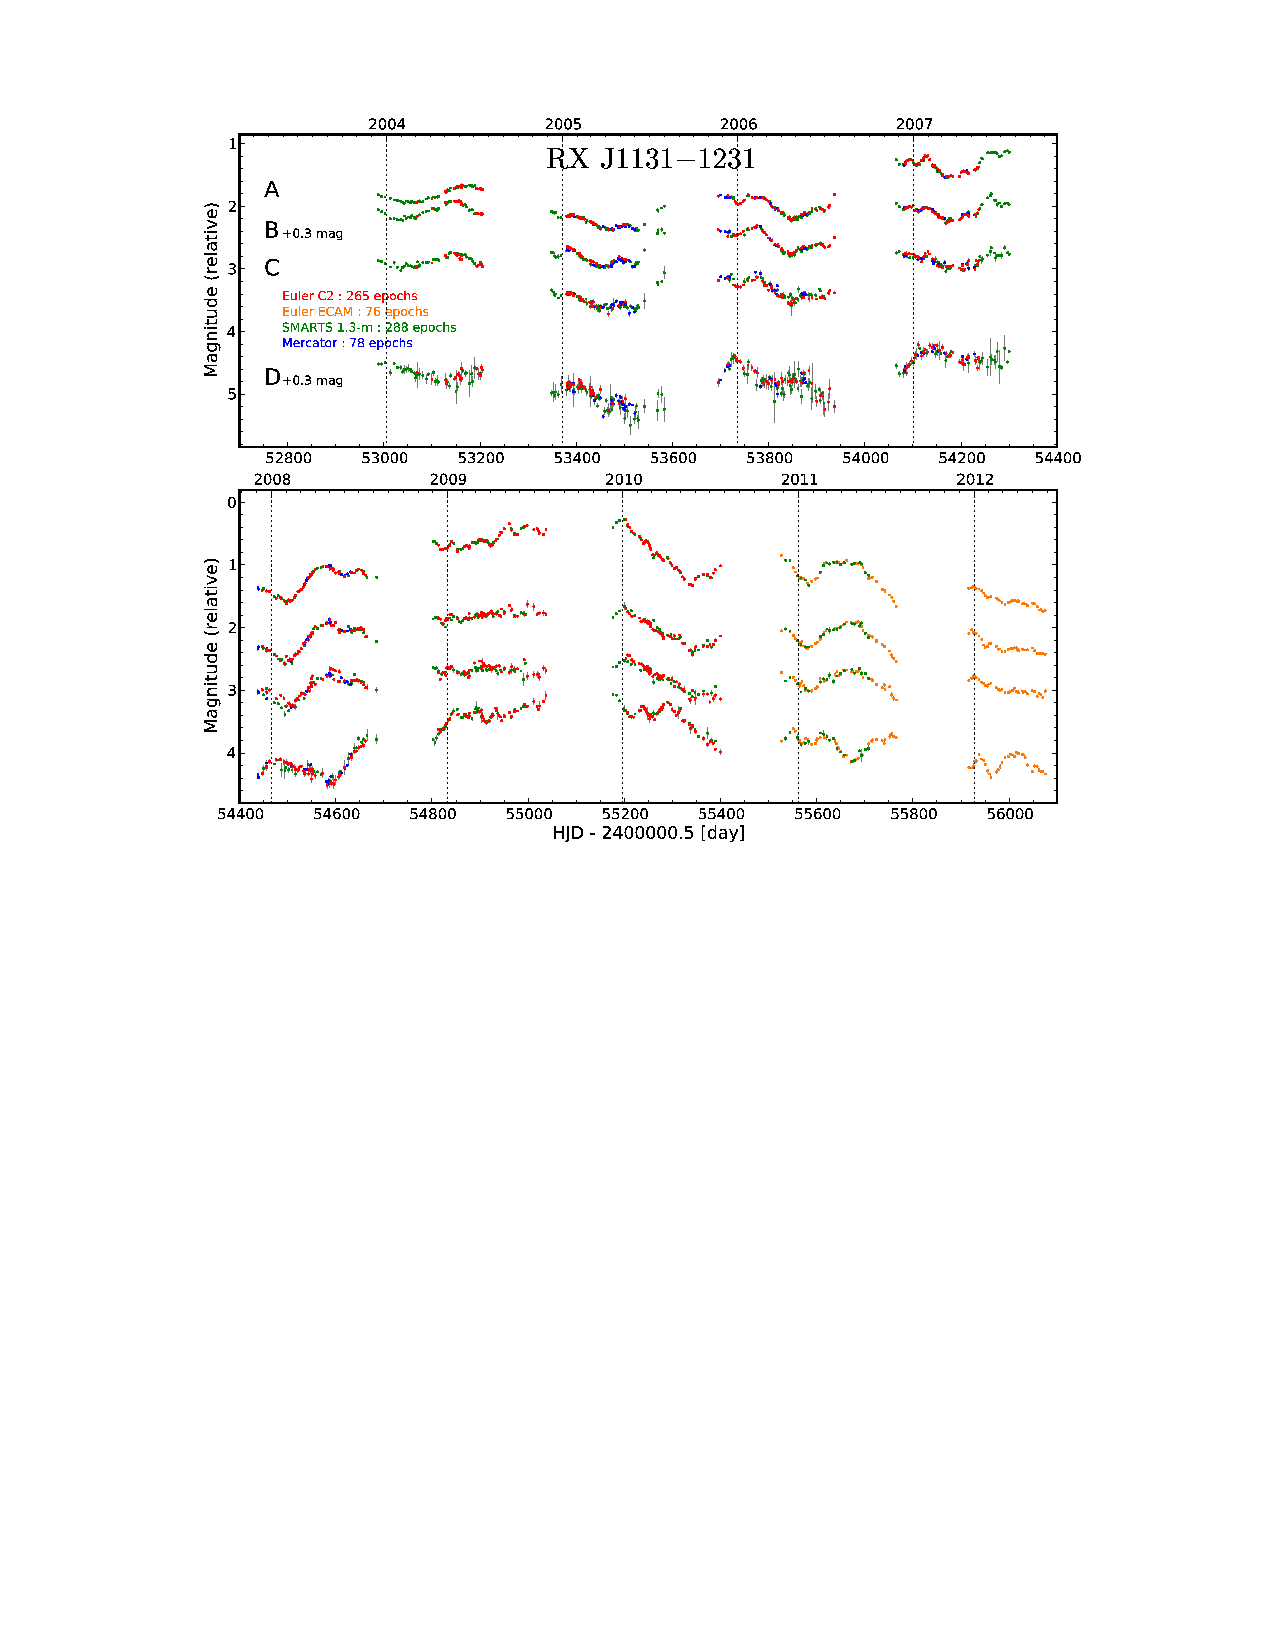
\includegraphics[width=0.48\textwidth]{figures/Tewes13-fig4.pdf}
\caption{Comparison between one of the early light curves \citep[left panel, from][]{Van89}, and a modern light curve from COSMOGRAIL \citep[right panel, from][]{Tew++13}. Note the improved photometric precision, cadence, and duration of the light curves, allowing for unambiguous determination of the time-delay to within 1-2\% precision.}
\label{fig:oldvsmoderndt}
\end{figure*}

Finally, when robust time delays started to become available, the
focus of the controversy shifted to the modeling of the gravitational
potential of the lens. Typically, in the mid ninenties, the only
constraints available to modelers were the quasar image positions and
to lesser extent flux ratios (limited by microlensing, variability and
differential extinction). Thus, the best one could do was to assume
some simple form for the lens potential like a singular isothermal
sphere \citep{K+F99}, thus breaking the mass sheet degeneracy, and to
neglect the effects of structure along the line of sight. Given these
necessary but oversimplistic assumptions, random errors grossly
underestimated the total uncertainty, leading to measurements
apparently inconsistent with those obtained by other groups or other
techniques
\citep{K+S04}. Since then, two methods have been pursued in order to
break degeneracies in more flexible modeling of the lensing data and
obtain realistic estimates on the uncertainties. One consists in using
large samples of systems with relatively weak priors
\citep{Ogu07b}. The other method consists in obtaining high quality data for
each lens system, such as detailed imaging of the quasar host galaxy
\citep{Keeton:2000p241,WBB04,Suy++06}, or non-lensing data like the deflector
stellar velocity dispersion \citep{T+K02b} and the properties of
galaxies along the line of sight \citep{K+Z04,Suy++10}. We discuss
these approaches in Section~\ref{ssec:lensmodel}. The astounding
improvement in data quality over the past two decades is illustrated
in Figure~\ref{fig:oldvsmodernimage}.

\begin{figure*}
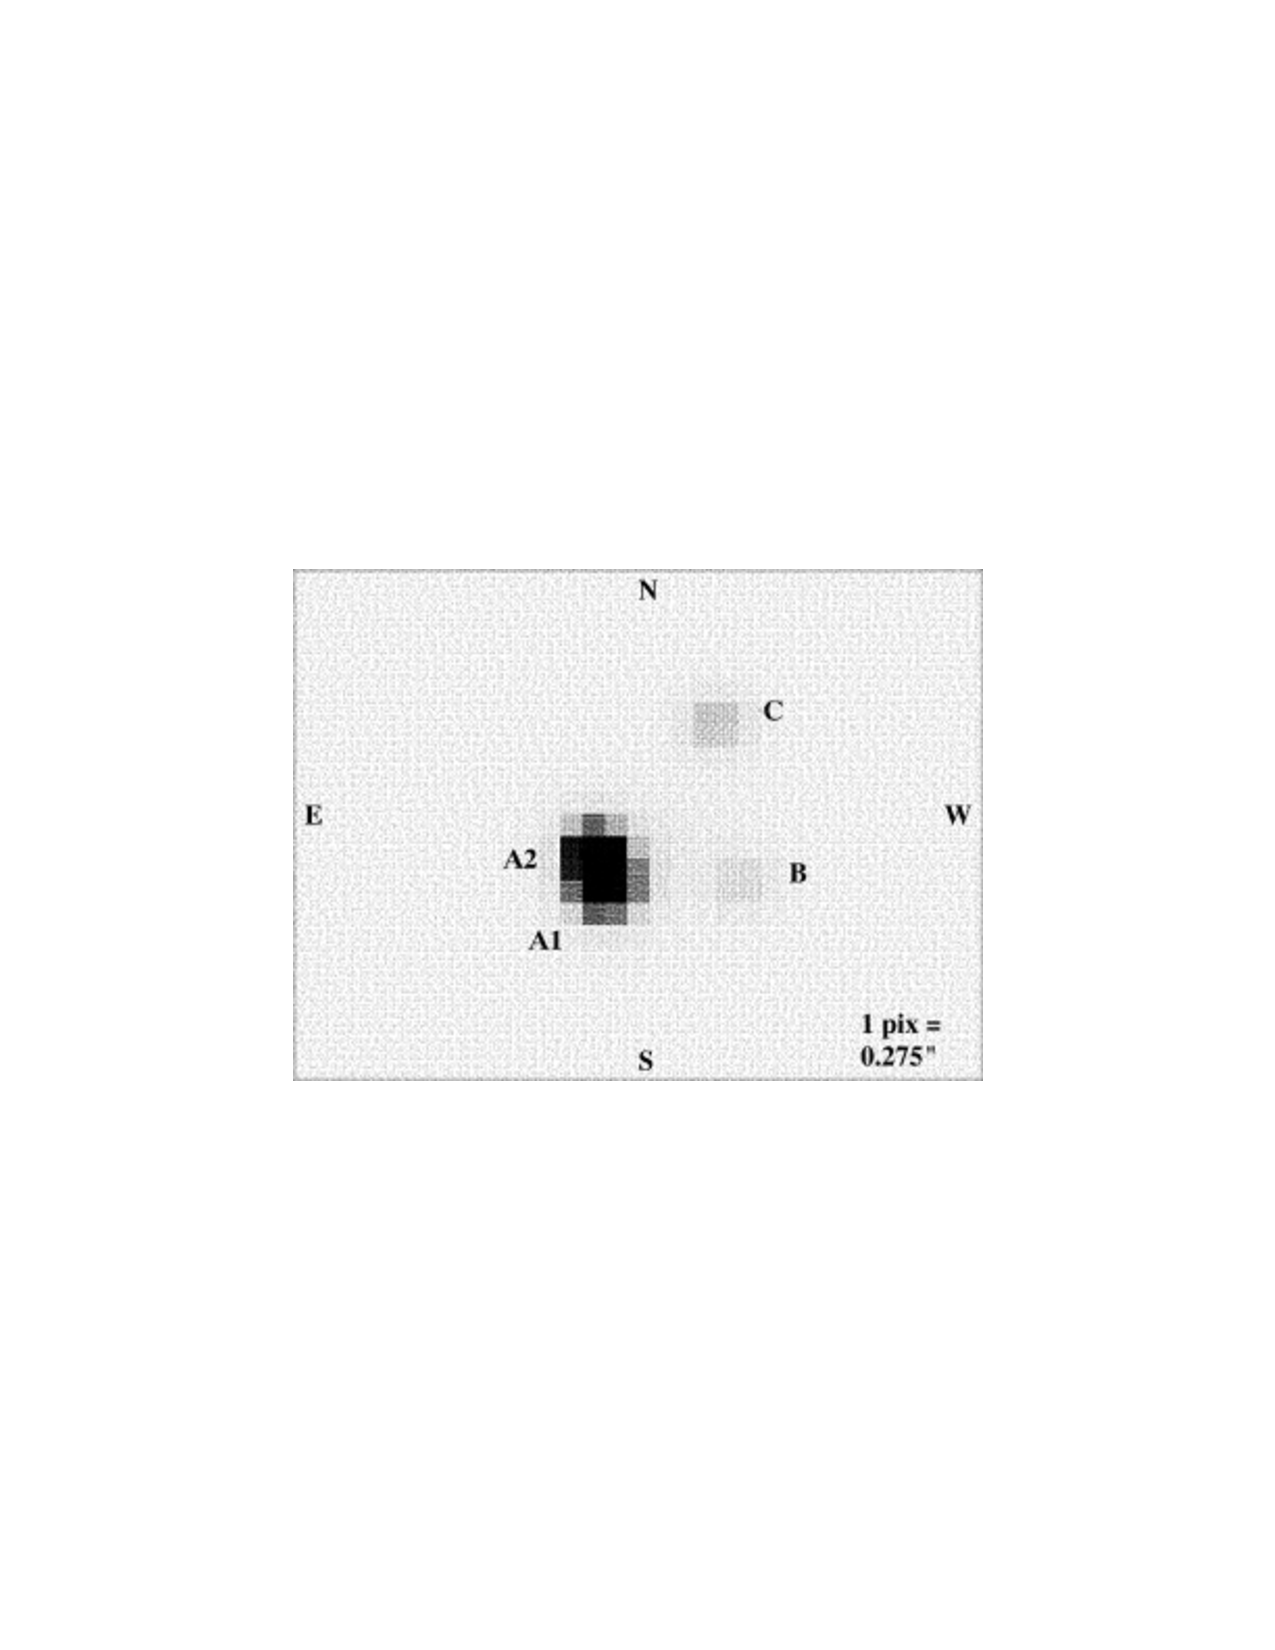
\includegraphics[height=3.5cm]{figures/Schechter97_fg1.pdf}
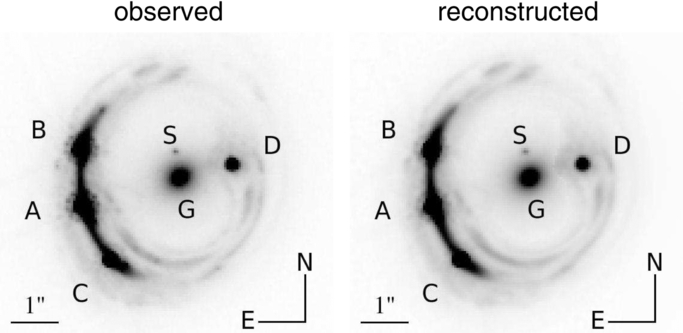
\includegraphics[height=3.5cm]{figures/Suyu14_fig1.jpg}
\caption{Comparison between imaging data available in the nineties \citep[eft panel, from][]{Sch++97} and in the most recent studies \citep[middle and right panels, from][]{Suy++14}). With modern data the structure of the quasar host galaxy can be modeled in great detail, providing thousands of constraints on the deflection angle, and thus on the derivatives of the gravitational potential.}
\label{fig:oldvsmodernimage}
\end{figure*}

Ultimately, the controversies over systematic errors were essential to
spur the community to overcome the difficulties and find ways to
address them. This is a natural and probably inevitable part of the
scientific process. However, the bitterness of some of those
controversies during the ninenties and early naughts still resonates
today. Unfortunately, some of the scientists that followed the field
with excitement at that time, are still under the impression that
strong lensing time delays are inherently inaccurate and imprecise. As
we have briefly described here, and we will discuss in detail in the
next sections, in the last twenty years the field has moved forward
considerably implementing many solutions to the lessons learned the
hard way.
